\documentclass[letterpaper]{article}
\usepackage{natbib}
\usepackage[utf8]{inputenc}
\usepackage{graphicx}
\usepackage{color}
\usepackage{multirow}
\usepackage{amsmath}
\usepackage{array}
\usepackage{subcaption}
\usepackage{mathpazo}
\usepackage[a4paper]{geometry}
\usepackage{float}

\title{Learning Dynamics: Assignment 3 \\
\Large Multi-Armed Bandits}
\author{\Large Hakim Boulahya \\ \\
Université Libre de Bruxelles \\
hboulahy@ulb.ac.be - 000391737
}

\begin{document}
\maketitle
\tableofcontents
\newpage

\section{N-Armed Bandit}


\subsection{Exercice 1}

% ex1 rewards
\begin{figure}[H]
    \centering
    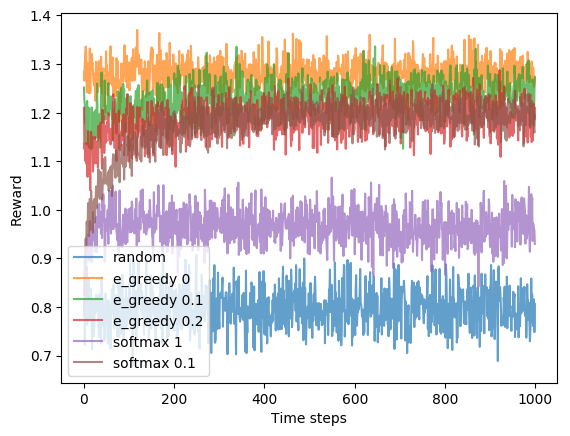
\includegraphics[width=.7\linewidth]{images/assign3/ex1/rewards}
    \caption{Average rewards for all algorithms}
    \label{fig:rewards_ex1}
\end{figure}


% ex1 qtas
\begin{figure}[H]
  \begin{subfigure}{.5\textwidth}
    \centering
    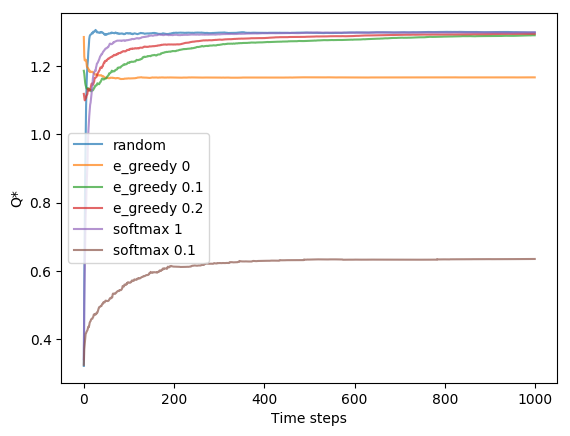
\includegraphics[width=1\linewidth]{images/assign3/ex1/qta_0}
    \caption{$Q_{a_{0}}(t)$}
    \label{fig:qta_0_ex1}
  \end{subfigure}
  \begin{subfigure}{.5\textwidth}
    \centering
    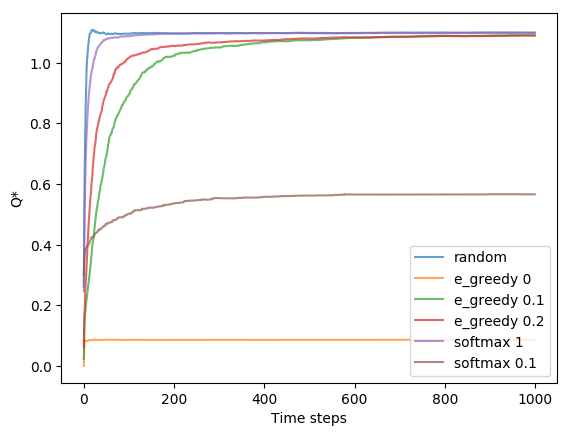
\includegraphics[width=1\linewidth]{images/assign3/ex1/qta_1}
    \caption{$Q_{a_{1}}(t)$}
    \label{fig:qta_1_ex1}
  \end{subfigure}
  \begin{subfigure}{.5\textwidth}
    \centering
    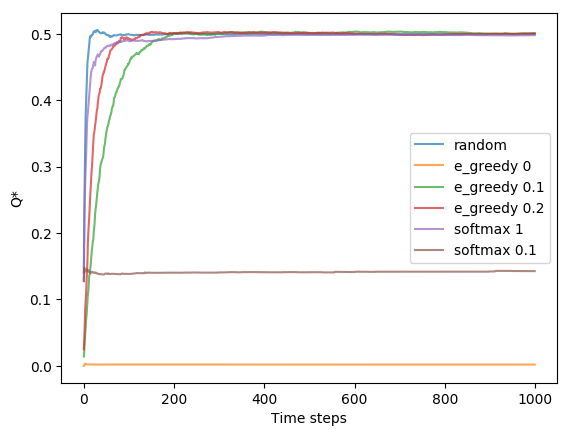
\includegraphics[width=1\linewidth]{images/assign3/ex1/qta_2}
    \caption{$Q_{a_{2}}(t)$}
    \label{fig:qta_2_ex1}
  \end{subfigure}
  \begin{subfigure}{.5\textwidth}
    \centering
    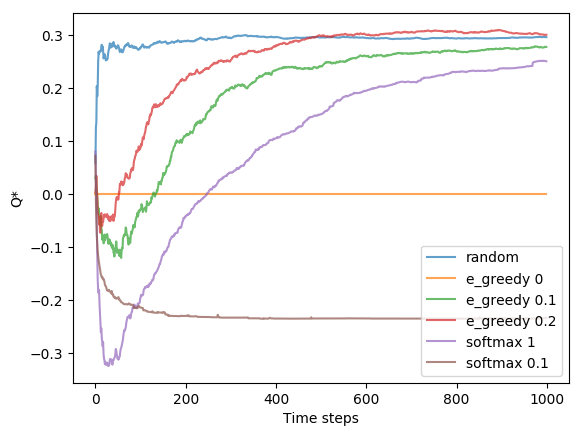
\includegraphics[width=1\linewidth]{images/assign3/ex1/qta_3}
    \caption{$Q_{a_{3}}(t)$}
    \label{fig:qta_3_ex1}
  \end{subfigure}

    \caption{Plot per arm showing
    the $Q^{*}_{a_{i}}$
    of that action along with the actual $Q_{a_{i}}$ a i estimate over time
    with
    $\mu$ = (1.3, 1.1, 0.5, 0.3), $\sigma$ = (0.9, 0.6, 0.4, 2.0)}
    \label{fig:qtas_ex1}
\end{figure}


% EX1 arms histograms
\begin{figure}[H]
  \begin{subfigure}{.5\textwidth}
    \centering
    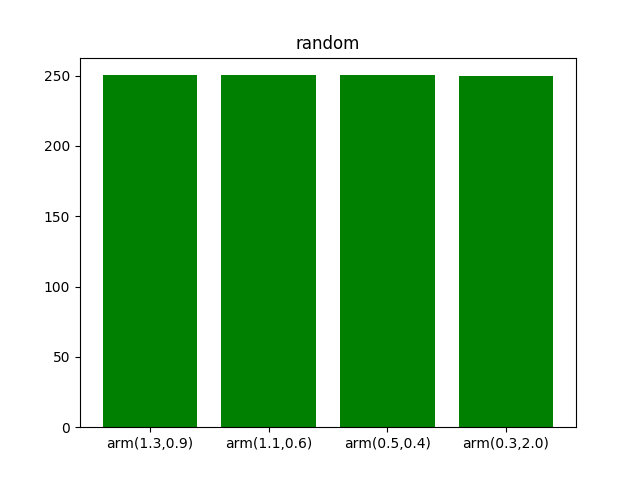
\includegraphics[width=1\linewidth]{images/assign3/ex1/arms_random}
    \caption{}
    \label{fig:arms_random_ex1}
  \end{subfigure}
  \begin{subfigure}{.5\textwidth}
    \centering
    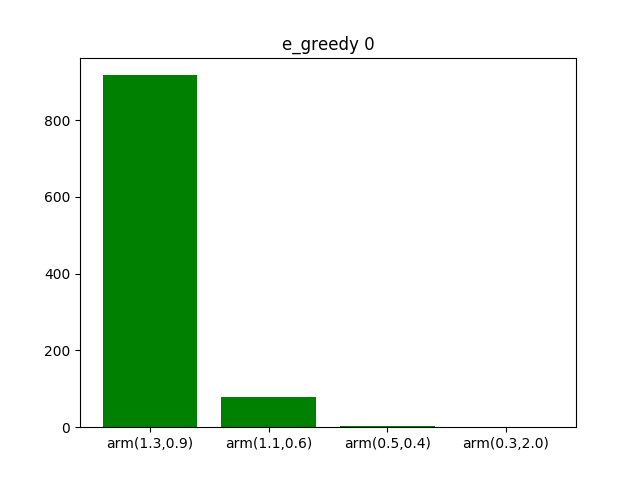
\includegraphics[width=1\linewidth]{images/assign3/ex1/arms_e_greedy0}
    \caption{}
    \label{fig:arms_e_greedy0_ex1}
  \end{subfigure}
  \begin{subfigure}{.5\textwidth}
    \centering
    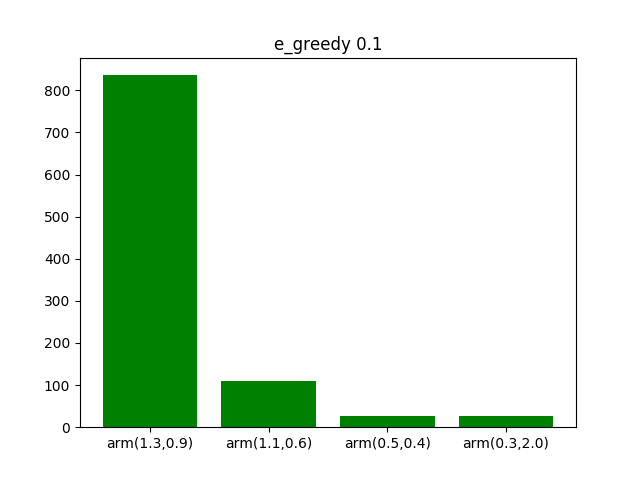
\includegraphics[width=1\linewidth]{images/assign3/ex1/arms_e_greedy01}
    \caption{}
    \label{fig:arms_e_greedy01_ex1}
  \end{subfigure}
  \begin{subfigure}{.5\textwidth}
    \centering
    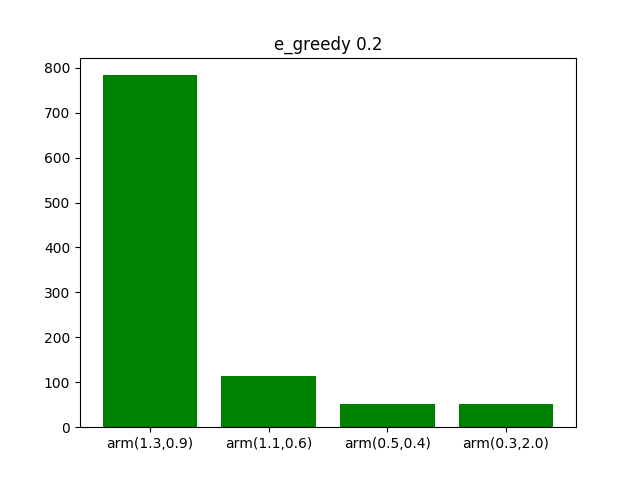
\includegraphics[width=1\linewidth]{images/assign3/ex1/arms_e_greedy02}
    \caption{}
    \label{fig:arms_e_greedy02_ex1}
  \end{subfigure}
  \begin{subfigure}{.5\textwidth}
    \centering
    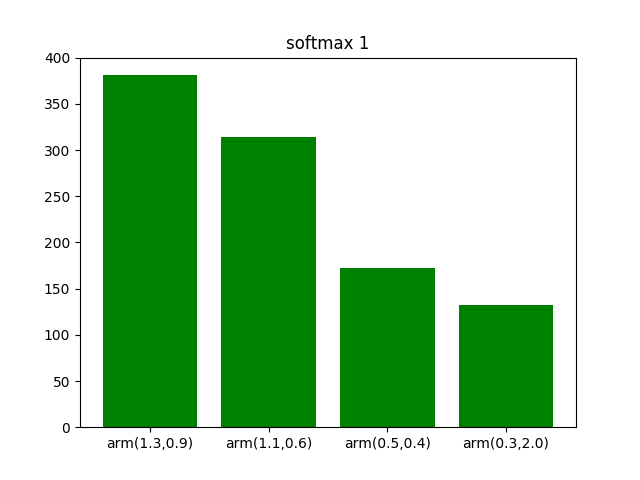
\includegraphics[width=1\linewidth]{images/assign3/ex1/arms_softmax1}
    \caption{}
    \label{fig:arms_softmax1_ex1}
  \end{subfigure}
  \begin{subfigure}{.5\textwidth}
    \centering
    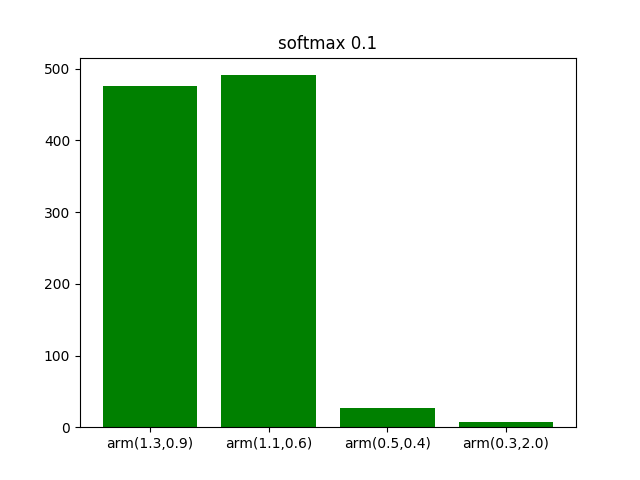
\includegraphics[width=1\linewidth]{images/assign3/ex1/arms_softmax01}
    \caption{}
    \label{fig:arms_softmax01_ex1}
  \end{subfigure}
    \caption{Histograms showing the number of times each action is selected
    per selection strategy with
    $\mu$ = (1.3, 1.1, 0.5, 0.3), $\sigma$ = (0.9, 0.6, 0.4, 2.0)}
    \label{fig:arms_ex1}
\end{figure}


\subsection{Exercice 2}

% ex2 rewards
\begin{figure}[H]
    \centering
    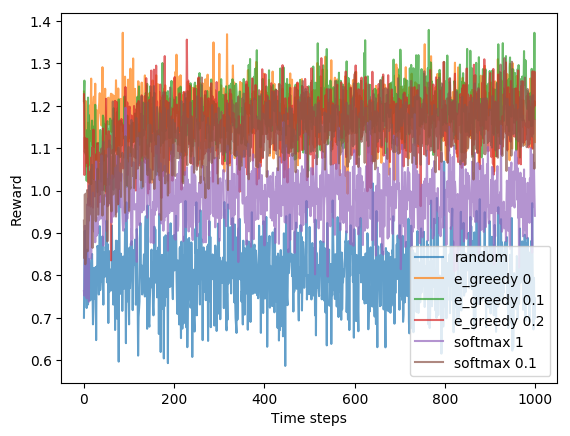
\includegraphics[width=.7\linewidth]{images/assign3/ex2/rewards}
    \caption{Average rewards for all algorithms}
    \label{fig:rewards_ex2}
\end{figure}


% ex2 qtas
\begin{figure}[H]
  \begin{subfigure}{.5\textwidth}
    \centering
    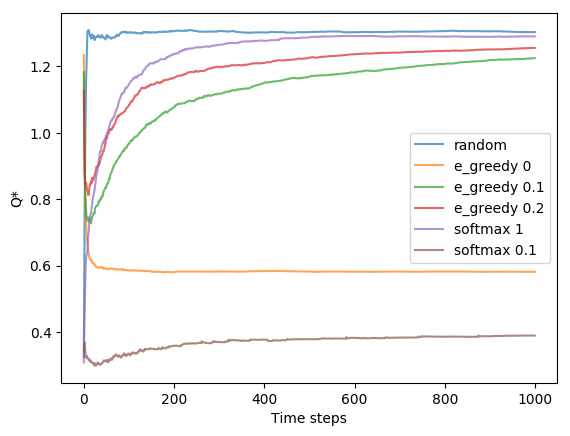
\includegraphics[width=1\linewidth]{images/assign3/ex2/qta_0}
    \caption{$Q_{a_{0}}(t)$}
    \label{fig:qta_0_ex2}
  \end{subfigure}
  \begin{subfigure}{.5\textwidth}
    \centering
    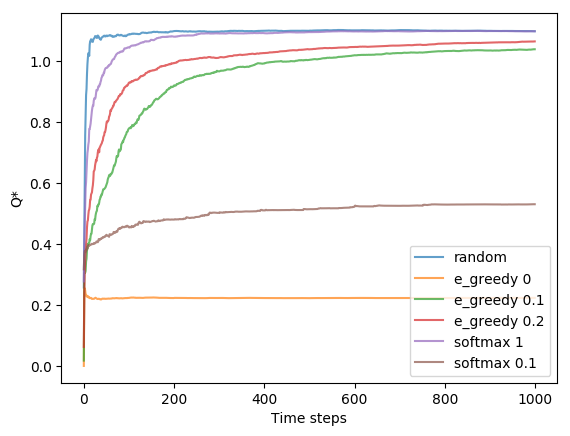
\includegraphics[width=1\linewidth]{images/assign3/ex2/qta_1}
    \caption{$Q_{a_{1}}(t)$}
    \label{fig:qta_1_ex2}
  \end{subfigure}
  \begin{subfigure}{.5\textwidth}
    \centering
    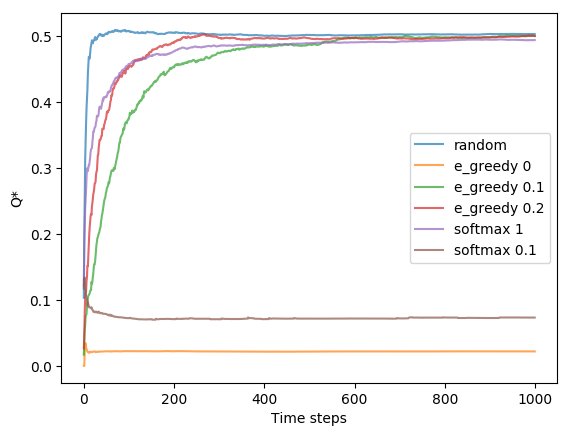
\includegraphics[width=1\linewidth]{images/assign3/ex2/qta_2}
    \caption{$Q_{a_{2}}(t)$}
    \label{fig:qta_2_ex2}
  \end{subfigure}
  \begin{subfigure}{.5\textwidth}
    \centering
    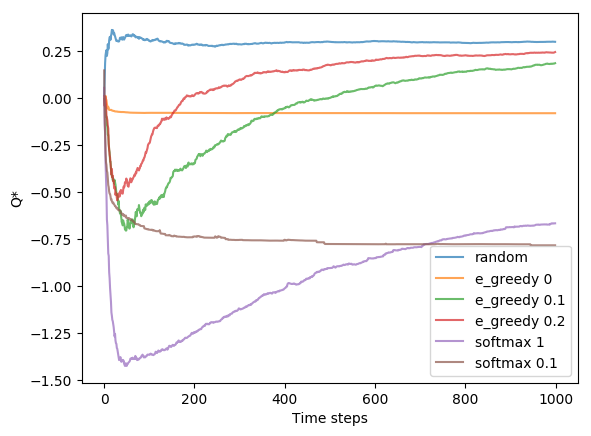
\includegraphics[width=1\linewidth]{images/assign3/ex2/qta_3}
    \caption{$Q_{a_{3}}(t)$}
    \label{fig:qta_3_ex2}
  \end{subfigure}

    \caption{Plot per arm showing
    the $Q^{*}_{a_{i}}$
    of that action along with the actual $Q_{a_{i}}$ a i estimate over time
    with
    $\mu$ = (1.3, 1.1, 0.5, 0.3), $\sigma$ = (1.8, 1.2, 0.8, 4.0)}
    \label{fig:qtas_ex2}
\end{figure}

% ex2 arms histograms
\begin{figure}[H]
  \begin{subfigure}{.5\textwidth}
    \centering
    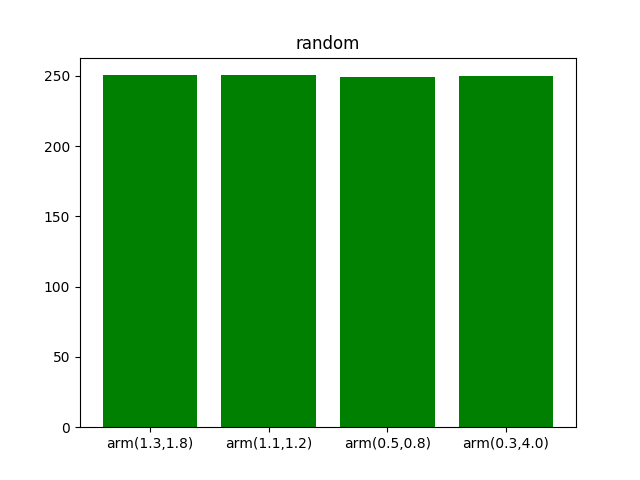
\includegraphics[width=1\linewidth]{images/assign3/ex2/arms_random}
    \caption{}
    \label{fig:arms_random_ex2}
  \end{subfigure}
  \begin{subfigure}{.5\textwidth}
    \centering
    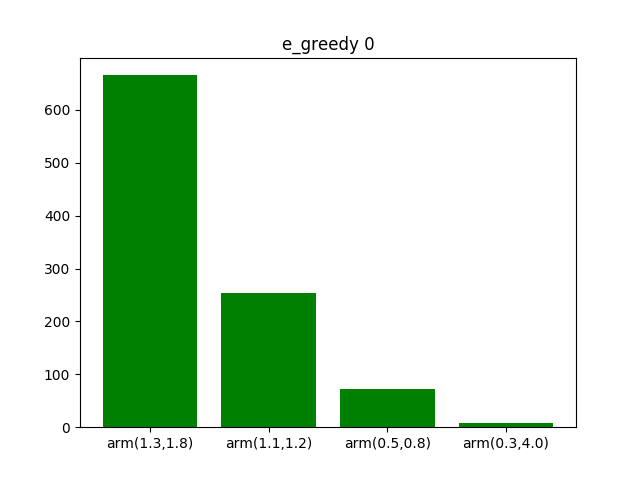
\includegraphics[width=1\linewidth]{images/assign3/ex2/arms_e_greedy0}
    \caption{}
    \label{fig:arms_e_greedy0_ex2}
  \end{subfigure}
  \begin{subfigure}{.5\textwidth}
    \centering
    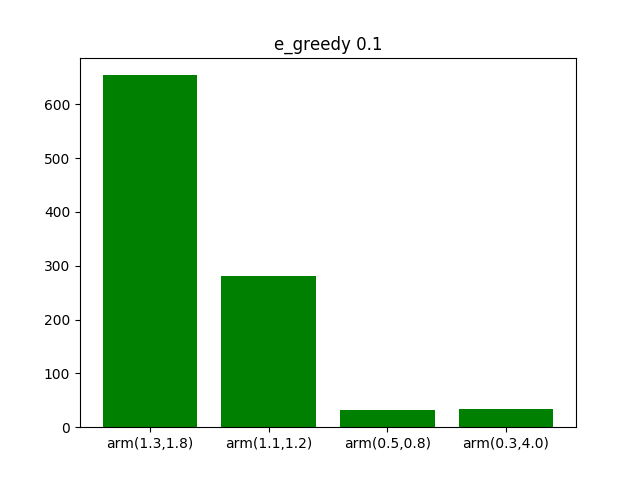
\includegraphics[width=1\linewidth]{images/assign3/ex2/arms_e_greedy01}
    \caption{}
    \label{fig:arms_e_greedy01_ex2}
  \end{subfigure}
  \begin{subfigure}{.5\textwidth}
    \centering
    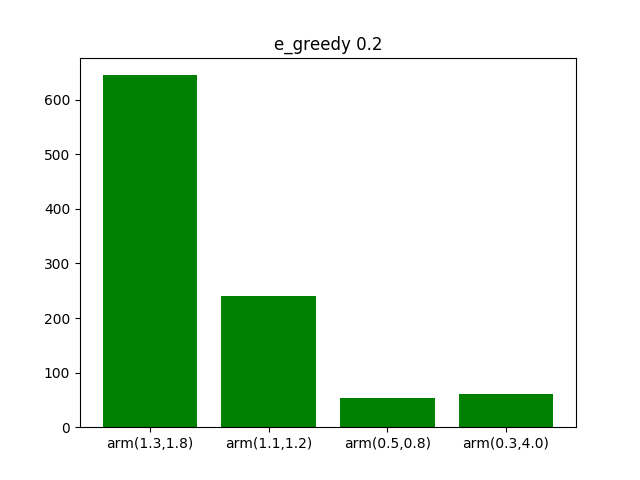
\includegraphics[width=1\linewidth]{images/assign3/ex2/arms_e_greedy02}
    \caption{}
    \label{fig:arms_e_greedy02_ex2}
  \end{subfigure}
  \begin{subfigure}{.5\textwidth}
    \centering
    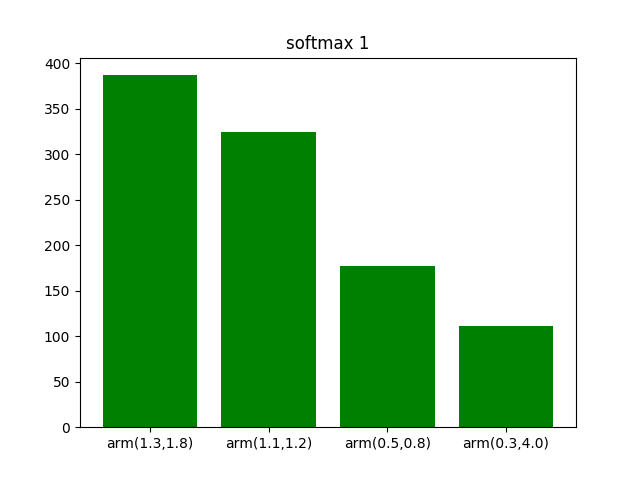
\includegraphics[width=1\linewidth]{images/assign3/ex2/arms_softmax1}
    \caption{}
    \label{fig:arms_softmax1_ex2}
  \end{subfigure}
  \begin{subfigure}{.5\textwidth}
    \centering
    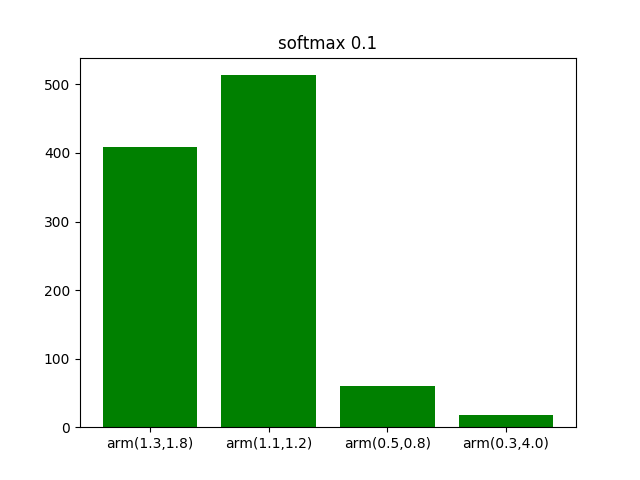
\includegraphics[width=1\linewidth]{images/assign3/ex2/arms_softmax01}
    \caption{}
    \label{fig:arms_softmax01_ex2}
  \end{subfigure}
    \caption{Histograms showing the number of times each action is selected
    per selection strategy with
    $\mu$ = (1.3, 1.1, 0.5, 0.3), $\sigma$ = (1.8, 1.2, 0.8, 4.0)}
    \label{fig:arms_ex2}
\end{figure}

\subsection{Exercice 3}

% ex3 rewards
\begin{figure}[H]
    \centering
    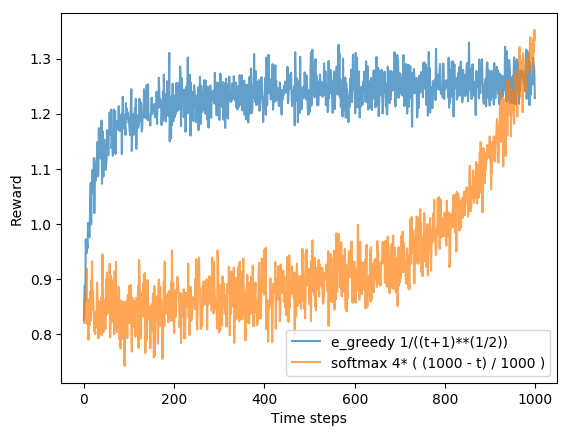
\includegraphics[width=.7\linewidth]{images/assign3/ex3/rewards}
    \caption{Average rewards for all algorithms}
    \label{fig:rewards_ex3}
\end{figure}


% ex3 qtas
\begin{figure}[H]
  \begin{subfigure}{.5\textwidth}
    \centering
    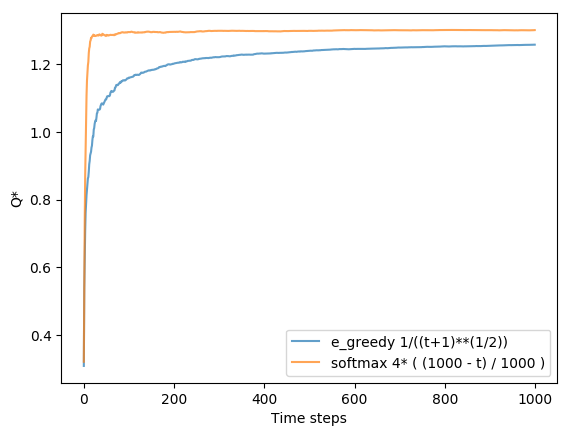
\includegraphics[width=1\linewidth]{images/assign3/ex3/qta_0}
    \caption{$Q_{a_{0}}(t)$}
    \label{fig:qta_0_ex3}
  \end{subfigure}
  \begin{subfigure}{.5\textwidth}
    \centering
    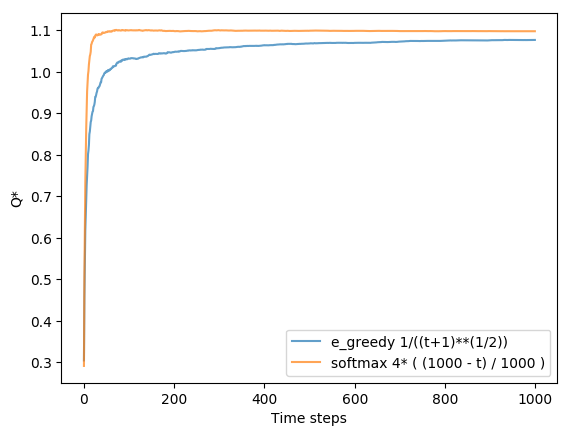
\includegraphics[width=1\linewidth]{images/assign3/ex3/qta_1}
    \caption{$Q_{a_{1}}(t)$}
    \label{fig:qta_1_ex3}
  \end{subfigure}
  \begin{subfigure}{.5\textwidth}
    \centering
    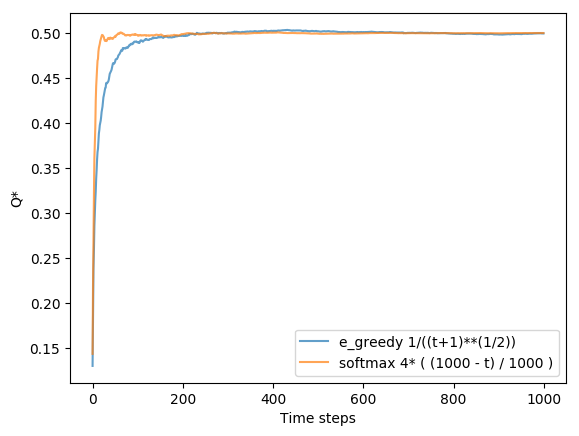
\includegraphics[width=1\linewidth]{images/assign3/ex3/qta_2}
    \caption{$Q_{a_{2}}(t)$}
    \label{fig:qta_2_ex3}
  \end{subfigure}
  \begin{subfigure}{.5\textwidth}
    \centering
    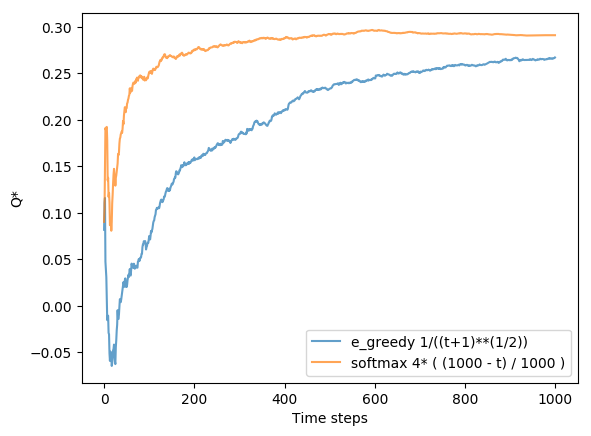
\includegraphics[width=1\linewidth]{images/assign3/ex3/qta_3}
    \caption{$Q_{a_{3}}(t)$}
    \label{fig:qta_3_ex3}
  \end{subfigure}

    \caption{Plot per arm showing
    the $Q^{*}_{a_{i}}$
    of that action along with the actual $Q_{a_{i}}$ a i estimate over time}
    \label{fig:qtas_ex3}
\end{figure}

% ex3 arms histograms
\begin{figure}[H]
    \begin{subfigure}{.5\textwidth}
    \centering
    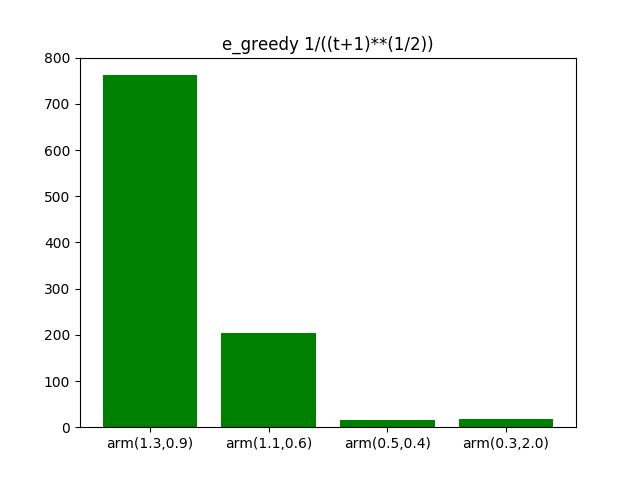
\includegraphics[width=1\linewidth]{images/assign3/ex3/arms_e_greedy_t}
    \caption{}
    \label{fig:arms_e_greedy_t_ex3}
    \end{subfigure}
    \begin{subfigure}{.5\textwidth}
      \centering
      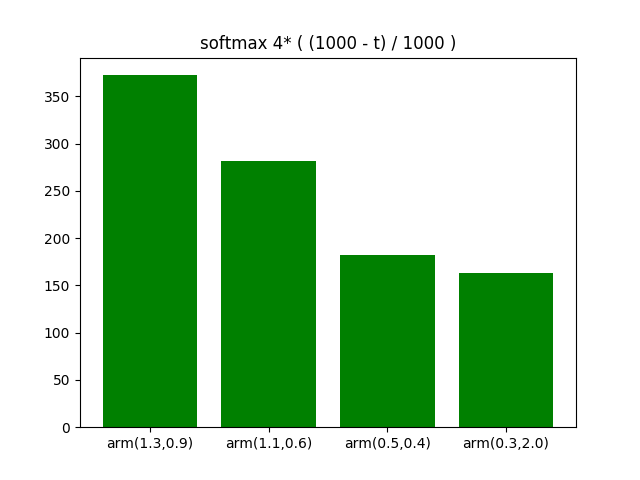
\includegraphics[width=1\linewidth]{images/assign3/ex3/arms_softmax_t}
      \caption{}
      \label{fig:arms_softmax_t_ex3}
    \end{subfigure}
    \caption{Histograms showing the number of times each action is selected
    per selection strategy}
    \label{fig:arms_ex3}
\end{figure}

\section{Climbing game}

When using the formula, it is important to have a big tau, because exp(Q/tau)
will give errors if Q is too big. (See how EV(a) is calculated)

I also remarked that when using EV with max_rewards or max_q when
min_tau = 0.001 the 11 is good, but when 0.1 or 1, not. THis is probably
due to the stochastic of our game.

\end{document}
